\documentclass[10pt]{article}         %% What type of document you're writing.

%%%%% Preamble

%% Packages to use

\usepackage{amsmath,amsfonts,amssymb,mathtools}   %% AMS mathematics macros
\usepackage{graphicx}
\usepackage[margin=1cm]{caption}
\usepackage{subcaption}
\usepackage{tikz}
\usepackage{cite}
\usetikzlibrary{decorations.pathreplacing,matrix}
\usetikzlibrary{decorations.pathmorphing}
\usetikzlibrary{decorations.text}

\tikzset{ 
  table/.style={
    matrix of math nodes,
    row sep=-\pgflinewidth,
    column sep=-\pgflinewidth,
    nodes={rectangle,text width=3em,align=center},
    text depth=1.0ex,
    text height=1.0ex,
    nodes in empty cells,
    left delimiter=[,
    right delimiter={]},
  }
}

\renewcommand{\labelenumi}{\arabic{enumi}.}
\renewcommand{\labelenumii}{\arabic{enumi}.\arabic{enumii}}

\DeclarePairedDelimiter\abs{\lvert}{\rvert}%
\DeclarePairedDelimiter\norm{\lVert}{\rVert}%
\newtheorem{exmp}{Example}[section]
%% Title Information.

\title{Monocular methods in stereo visual odometry}
\author{Ilan Shimshoni, Ehud Rivlin, Alex Kreimer}

\begin{document}

\maketitle

\abstract{We propose a new algorithm for stereo visual odometry based on monocular methods}

\section{Questions}
What is the influence of the far away points on the 3d based
algorithms?  ~\cite{tardif2008monocular} claim that since they may not
be reliably reconstructed these points are a burden and thus it is an
advantage of epipolar geometry based methods.

\section{Introduction}

\section{Related Work}

\section{Image Features}

\section{Image Point Mapping Related to Camera Motion}

Suppose the camera matrices are those of a calibrated stereo rig with
the world origin at the first camera

\[
\mathrm{P = K[I\ |\ 0]\quad P'=K'[R\ |\ \mathbf{t}]}
\]

Consider projections of a 3D point $(X,Y,Z,1)^T$ into the image planes of both views:

\[
\mathrm{\mathbf{x} = P\mathbf{X} \quad \mathbf{x}' = P'\mathbf{X}}
\]

If the image point is normalized as $\mathbf{x} = (x,y,1)^T$ then
\[
\mathbf{x}Z = \mathrm{P\mathbf{X} = K[I\ |\ 0]\mathbf{X} = K}(X,Y,Z)^T
\]

It follows that $(X,Y,Z)^T = \mathrm{K^{-1}}\mathbf{x}Z$, and:
\begin{align*}
  \mathbf{x}' &= \mathrm{K'[R\ |\ \mathbf{t}]}(X,Y,Z,1)^T \\
  &= \mathrm{K'R}(X,Y,Z)^T + \mathrm{K'\mathbf{t}}\\
  &= \mathrm{K'RK^{-1}}\mathbf{x}Z + \mathrm{K'\mathbf{t}}\\
\end{align*}

Now we divide both sides by $Z$ to obtain the mapping of an image point $\mathbf{x}$ to image point $\mathbf{x}'$
\[
\mathbf{x}' = \mathrm{K'RK^{-1}}\mathbf{x} + \mathrm{K'}\mathbf{t}/Z = \mathrm{H}\mathbf{x}+ \mathrm{K'}\mathbf{t}/Z
\]

If $\mathrm{R = I}$ (e.g. pure translation) the point $\mathbf{x}$ will undergo a motion along a corresponding epipolar line:
\[
\mathbf{x}' = \mathbf{x}+ \mathrm{K'}\mathbf{t}/Z = \mathbf{e}'/Z
\]

If $\mathbf{t} = \mathbf{0}$ the motion of the point may be represented by a homology:
\[
\mathbf{x}' = \mathrm{H}\mathbf{x}
\]

\begin{figure}[h]
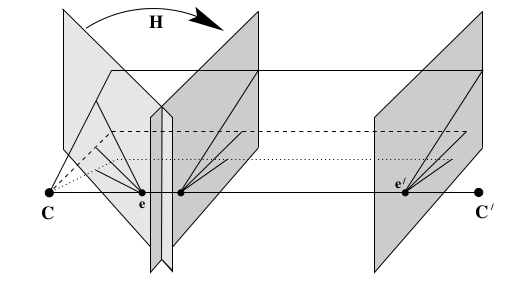
\includegraphics[scale=.5]{general_camera_motion}
\centering
\caption{General camera motion may be viewed as a two step process}
\end{figure}

In a general case the mapping of an image point $\mathbf{x}$ into $\mathbf{x}'$ may be viewed as a two step process: transformation by a homology (a specialization of homography which has two equal eigenvalues) $\mathrm{H}$ which simulates a pure rotational motion of the camera followed by an offset along the epipolar line which simulates a pure translational motion of the camera.

\section{Estimation of Camera Rotation}
We would like to exploit the fact that for $Z \gg \mathbf{\norm{t}}_2$
\[
\mathbf{x}' \approx \mathrm{H}\mathbf{x}
\]
\section{Monocular motion estimation}\label{sec:mono_odo}
Let $C_1$ and $C_2$ be the two camera frames.  $R$ describes the
orientation of $C_1$ in as seen from $C_2$. $t_1$ is a direction (line
of site of the origin) from $C_2$ to $C_1$ described in $C_2$ (see
Figure ~\ref{fig:two_views}).  We are interested to recover $R$ and
$t$ from image feature measurements.

\subsection{Fundamental Matrix Estimation}
First method that we consider estimates Fundamental matrix:
\begin{enumerate}
\item Estimate the Fundamental matrix $\mathbf{F}$. We use normalized 8-point algorithm.
\item Recover the Essential matrix: $\mathbf{E} = K^T\mathbf{F}K$
\item Decompose $\mathbf{E}$ into camera rotation and translation, s.t. $\mathbf{E} = [\mathbf{t}]_\times\mathbf{R}$.
\item Use non-linear optimization to improve the result.
\end{enumerate}

\subsection{Experimental Comparison of Motion Parameter Refinement Methods}

Thus for every pair of image correspondences $x\in C_1,x'\in C_2$ holds
\[
x'^TK^{-1}[q]_{\times}RK^{-1}x=0
\]
where $K$ is an intrinsic parameters matrix and $E=[q]_{\times}R$ is
the essential matrix.  We estimate the fundamental
($F=K^{-1}[q]_{\times}RK^{-1}$) using a standard technique such as
normalized 8-point algorithm) and then strip it down to essential
matrix.  Further on we decompose the essential to obtain motion
parameters $q$ and $R$.  $R$ may be determined exactly while $q$ only
up to scale There are 4 different decompositions, which produce the
same essential, but only one is correct.  This ambiguity is resolved
by imposing the chierality constraint upon the scene points.

An in-depth review of fundamental matrix and its uncertainty
estimation is given in ~\cite{zhang1998determining}

\begin{figure}[!h]
  \centering
  \begin{tikzpicture}
    \draw [help lines, dotted] (0,0) grid (4,3); \draw [dashed] (0,0)
    -- (2,2); \draw [->] (2,2) -- (1.5,1.5); \node [left] at (1.5,1.5)
    {$R,q_1$}; \draw [red, fill] (0,0) circle [radius=0.05]; \node
    [below left] at (0,0) {$C_1$}; \node [above left] at (2,2)
    {$C_2$}; \draw [red, fill] (2,2) circle [radius=0.05];
  \end{tikzpicture}
  \caption{Two views}
  \label{fig:two_views}
\end{figure}

\section{Sensitivity of epipole estimation}
We search for a way to estimate camera motion direction (e.g. the
epipole) given a pair of overlapping views.  Follows the outline of
two methods that we analyze.  Both methods rely on a set of putative matches that were extracted 

\item Method 2:
\begin{enumerate}
\item Estimate homography $\mathbf{H}_{\boldsymbol{\infty}}$
\item Warp homography estimation outliers using
  $\mathbf{H}_{\boldsymbol{\infty}}$ (this cancels the influence of
  orientation difference between two given views and leaves
  only the influence of translation)
\item Compute the epipole $\mathbf{e}$.  The epipole is the vanishing
  point of the epipolar lines. Since the motion is pure translation
  the features move along the epipolar lines. We fit lines into the
  corresponding line segments and force all of them to intersect at
  the same point ($\mathbf{e}$).  We do this by minimizing the
  orthogonal distances from the epipolar lines to the corresponding
  feature points (MLE). Consider notation:
  \begin{enumerate}
  \item $a_i, b_i$ are the image coordinate of the feature point $i$
    in the second view
  \item $n_i$ is the normal vector in the image plane to the epipolar
    line that passes through $a_i,b_i$ 
  \item $l_i$ is this epipolar line
  \item $d(l_i,x)$ is the orthogonal distance between $l_i$ and $x$
  \item $e$ is the epipole or a vanishing point that all the epipolar
    lines intersect in
\end{enumerate}
\[
\underset{\{n_i\}_{i=1}^n,e}{\text{argmin}}\ \sum_{i=1}^nd^2(l_i,a_i) + d^2(l_i,b_i)\quad\text{s.t.} \sum_{i=1}^nd(l_i,e)=0
\]
\end{enumerate}
The main difference between two methods is that the former estimates
all motion parameters at once while the latter does it in two steps.

Below we provide the details of the experimental setup and its results

\subsection{Experimental setup}

We generate $N$ 3d points that are uniformly spread at
$[-z_{min};z_{max}]$ in front of the camera.  The camera translates
$1$m in positive $z$-direction.  Normal Gaussian noise is added to
feature point locations in the second view and then we use each one of
the methods described in previous section to recover the epipole.

\section{Algorithm Description}

The algorithm in ~\ref{algo} solves VO in stereo setting. It relies on
the estimation and decomposition of the essential matrix and the
invariance of the cross-ratio under projectile transformation so we
overview these first in ~\ref{sec:mono_odo} and ~\ref{sec:cross_ratio}


\subsection{Cross-ratio}\label{sec:cross_ratio}

We propose to exploit the fact that most of the time the car goes more
or less straight forward.  This special case of camera motion
possesses peculiar cross-ratio related properties.

It is a known fact ~\cite{Hartley2004} that if camera motion is a pure
translation the projections of the world point will ``surf'' along the
epipolar line (towards the epipole or away from it depending on the
sign of the translation vector). It was also shown
~\cite{basri1999visual} that the cross ratio of feature locations and
the vanishing point is exactly the same as the one of the camera
centers and the ideal point and thus may be used as an additional
constraint in motion estimation.

We face two issues: decide when to use the cross ratio constraint and
how to incorporate it into the motion estimation process.

To address the first question we fit a line into the three last
feature locations and use the residuals to make a decision.  Thus,
given a triplet of (homogeneous) feature locations $p_i,p'_i,p''_i$ and the epipole
$e$ (see figure ~\ref{fig:cross_ratio}) we fit a line $w\in R^3$ by solving linear orthogonal regression (using QR decomposition and SVD):

\[
w_i^* = \underset{w}{\text{argmin}} \ \norm{A_iw_i}_2\ \text{s.t.}\
w^2_i[1]+w^2_i[2]=1
\]

where $A_i=[p_i,p'_i,p''_i,e]^T$.  The residuals are given by (the
summation is over all the features that are available in last three
images):
\begin{equation}\label{eq:puret}
  \hat{r}_t = \frac{1}{N} \sum_{i=1}^N A_iw_i^*
\end{equation}

Thus the value of $\hat{r}_t$ may be used to quantitatively assess how
``purely translational'' is the motion at time $t$.

The cross ratio for feature point $i$ is given by:
\[
Cr(p_i,p'_i,p''_i,e) =
\frac{\norm{p''_i-p_i}\norm{e-p'_i}}{\norm{p'_i-p_i}\norm{e-p''_i}}
\]
Let $O,O',O''$ be the centers of the cameras for $p_i,p'_i,p''_i$
respectively and let $V_\infty$ be the ideal point of camera motion.
Thus for every feature point $i$ holds:
\[
Cr(O,O',O'',V_{\infty}) = Cr(p_i,p'_i,p''_i,e) \;
\]

Let us denote $Cr_t = Cr(O,O',O'',V_{\infty})$.

Since the locations of the features are noisy we compute average
cross-ratio value:
\[
\hat{Cr} =  \frac{1}{N}\sum_{i=1}^NCr(p_i,p'_i,p''_i,e) \;
\]

And thus for time $t$ we have:
\begin{equation}\label{eq:cr}
  Cr_t = \hat{Cr}
\end{equation}

We will use both ~\ref{eq:puret} and ~\ref{eq:cr} in the motion
parameter fitting procedure.

\begin{figure}[!h]
  \centering
  \begin{tikzpicture}
    \draw [help lines, dotted] (0,0) grid (6,3); \draw [->] (0,0) --
    (5,3); \draw [green, fill] (0,0) circle [radius=0.02]; \draw
    [green, fill] (1,.6) circle [radius=0.02]; \draw [green, fill]
    (3.35,2) circle [radius=0.02]; \draw [green, fill] (5,3) circle
    [radius=0.02]; \node [above left] at (0,0) {$p_i$}; \node [above
    left] at (1,.6) {$p'_i$}; \node [above left] at (3.35,2) {$p''_i$};
    \node [above left] at (5,3) {$e$};
  \end{tikzpicture}
  \caption{Feature motion feature along the epipolar line during
    camera translation.  The cross ratio $Cr(p_i,p'_i,p''_i,e) =
    \frac{\norm{p''_i-p_i}\norm{e-p'_i}}
    {\norm{p'_i-p_i}\norm{e-p''_i}}$ has the same value for all
    features in the image.}
  \label{fig:cross_ratio}
\end{figure}

\subsection{Stereo setup}

\subsubsection{Stereo motion estimation}\label{algo}

\paragraph{Problem statement} Let $C_t/C_t' \in \mathbf{SE}(3) $
denote the pose of the left/right camera (respectively) at time $t$ as
seen in the world coordinate frame (usually placed at $C_1$). The rig is
moving rigidly, i.e., there is $T_t \in \mathbf{SE}(3)$ s.t. $ C_t =
T_t*C_{t-1}; C'_t = T_t*C'_{t-1}$ (see Figure ~\ref{fig:stereo_rig}).
Our goal is to estimate $T_t$ given the images taken by the camera at
times $\{t,t-1 \ldots t-k\}$

The algorithm presented in ~\ref{sec:mono_odo} may determine
rotation completely and translation up to scale.  In case of a stereo
rig we can also determine the scale of the translation.  Below is the
algorithm outline:

\subsection{Shortest distance between skew lines}\label{skew}
Consider two lines $l_1,l_2$ specified by points $P_1,P_2$ and directions
$\mathbf{v_1},\mathbf{v_2}$ respectively.

General point on $l_1$ is: $\hat{P_1}=P_1+t_1\mathbf{v_1}$, on $l_2$:
$\hat{P_2}=P_2+t_2\mathbf{v_2}$.

Consider vector $\hat{P_2}\hat{P_1} = P_2-P_1+t_2\mathbf{v_2}-t_1\mathbf{v_1}$

We are looking for such $\hat{P_2}\hat{P_1}$ that is orthogonal to both $\mathbf{v_1}$ and $\mathbf{v_2}$.
\[
\begin{array}{lcl}
   \hat{P_2}\hat{P_1}^T\mathbf{v_1} & =  P_2^T\mathbf{v_1}-P_1^T\mathbf{v_1} + t_2\mathbf{v_2}^T\mathbf{v_1}-t_1\mathbf{v_1}^T\mathbf{v_1} = & 0 \\
   \hat{P_2}\hat{P_1}^T\mathbf{v_2} & = P_2^T\mathbf{v_2}-P_1^T\mathbf{v_2} + t_2\mathbf{v_2}^T\mathbf{v_2}-t_1\mathbf{v_1}^T\mathbf{v_2} = & 0
\end{array}
\]

In matrix notation:
\[
\begin{bmatrix}
-\mathbf{v_1}^T\mathbf{v_1} & \mathbf{v_2}^T\mathbf{v_1} \\
-\mathbf{v_1}^T\mathbf{v_2} & \mathbf{v_2}^T\mathbf{v_2} \\
\end{bmatrix}
\begin{bmatrix}
t_1 \\ t_2 
\end{bmatrix}=
\begin{bmatrix}
P_2^T\mathbf{v_1}-P_1^T\mathbf{v_1} \\ P_2^T\mathbf{v_2}-P_1^T\mathbf{v_2} 
\end{bmatrix}
\]

\paragraph{Algorithm 1 (initial estimate)}
\begin{enumerate}
\item Estimate $T_t=[R_t,q_t]$ using the algorithm in ~\ref{sec:mono_odo}
\item Estimate $T'_t=[R'_t,q'_t]$ the same way
\item Use \ref{skew} to find the point closest to both lines of sight.
\end{enumerate}

\begin{figure}[!h]
  \centering
  \begin{tikzpicture}
    \draw [help lines, dotted] (0,0) grid (6,3); \draw [dashed] (0,0)
    -- (2,2); \draw [dashed] (3,0) -- (2,2); \draw [->] (0,0) --
    (.5,.5); \node [left] at (.5,.5) {$T_t=[R_t,q_t]$}; \draw [->] (3,0) --
    (2.75,.5); \node [right] at (2.75,.5) {$T'_t=[R'_t,q'_t]$}; \draw [red, fill]
    (0,0) circle [radius=0.05]; \draw [blue, fill] (3,0) circle
    [radius=0.05]; \node [below left] at (0,0) {$C_{t-1}$}; \node [below
    right] at (3,0) {$C_{t-1}'$}; \node [above left] at (2,2) {$C_t$};
    \node [above right] at (5,2) {$C_t'$}; \draw [red, fill] (2,2)
    circle [radius=0.05]; \draw [blue, fill] (5,2)
    circle [radius=0.05];
  \end{tikzpicture}
  \caption{Motion of a stereo rig}
  \label{fig:stereo_rig}
\end{figure}

\subsection{Reprojection error minimization}
Parameter sensitivity issues, especially in (X,Y,Z)...

\subsection{Essential Matrix refinement step}

We follow approach proposed in ~\cite{Botterill-etal-2011c} to refine
camera motion parameters. Let $r_i(E)$ be the Sampson's error
approximation:

\[
r_i(E) = \frac{x_i'^TEx_i}{\sqrt{(x_i'^TE)^2_0+(x_i'^TE)^2_1+(Ex_i)^2_0+(Ex_i)^2_1}}
\]

If point localization errors are approximately Gaussian, given N
correctly matched features $\{(x_i,x_i') | i=1\ldots N\}$ the MLE of E is approximately
the point where $\sum_{i=1}^{N} r_i(E)^2$ is minimized.

It is common to minimize functions in the form of sum of squares using
the Levenberg-Marquardt (LM) algorithm ~\cite{marquardt1963algorithm},
a dynamically damped version of Gauss-Newton.  It is also common to
use robust cost functions to cope with outliers (which break Gaussian
residual assumption).  This is known as Iteratively Reweighted Least
Squares, or IRLS ~\cite{Hartley2004}.  To minimize a function
$\sum_{i=1}^N C(r_i)$ for an arbitrary cost function C using IRLS,
weights $\{w_i\}$ are chosen so that $(w_ir_i)^2=C(r_i)$. The function
$\sum_{i=1}^N (w_ir_i)^2$ is minimized by LM, with weights recomputed
at each iteration.

$E$ is parameterized as a function $E(q,t)$ of a unit translation
vector $t$, and a rotation, which is expressed as a quaternion
$q$. Unit quaternions represent 3D rotations as 4D vectors. 4D unit
vectors form the differential manifold $\mathbb{S}^3$ (a unit sphere
in $R^4$).

At each iteration, the manifold $\mathbb{S}^3$ is parameterized as
three orthogonal vectors $\tau_1,\tau_2,\tau_3$ tangent to the sphere
$\mathbb{S}^3$ at $q$.  For each correspondence $(x_i,x_i')$, the
derivative of the cost function in the direction $\tau_j$ is computed
by finite differences.

\subsection{Non-linear refinement and use of cross-ratio}
Now we use non-linear optimization to refine the results and
incorporate cross-ratio information.

\subsection{Option 1: constant directions $\mathbf{q_t}, \mathbf{q_{t+1}}$}

Denote the direction of left camera motion relative to the previous
left (right) camera by (unit vectors) $\mathbf{q_t},\mathbf{q_{t+1}}$
($\mathbf{q'_t},\mathbf{q'_{t+1}}$) and its magnitude by $c_t,c_{t+1}$
($c'_t,c'_{t+1}$) at times $t$ and $t+1$ respectively (see
Fig. \ref{fig:cross_ratio_refine})

\begin{figure}[!h]
  \centering
  \begin{tikzpicture}
    \draw [help lines, dotted] (0,0) grid (8,6); \draw [dashed] (0,0)
    -- (2,2); \draw [dashed] (3,0) -- (2,2); \draw [dashed] (2,2) --
    (4,4); \draw [dashed] (4,4) -- (5,2); \draw [dashed,->] (3,0) --
    (0.05,0); \draw [dashed,->] (5,2) -- (2.05,2); \draw [->] (0,0) --
    (.5,.5); \draw [->] (2,2) -- (2.5,2.5); \node [left, scale=.7] at
    (0,.5) {$[R_t,q_t]$}; \node [left, scale=.7] at (2.3,2.8)
    {$[R_{t+1},q_{t+1}]$}; \draw [->] (3,0) -- (2.75,.5); \draw [->]
    (5,2) -- (4.423,3.15); \node [right, scale=.7] at (3.25,.5)
    {$[R'_t,q'_t]$}; \draw [red, fill] (0,0) circle [radius=0.05];
    \draw [red, fill] (4,4) circle [radius=0.05]; \draw [blue, fill]
    (3,0) circle [radius=0.05]; \node [below left] at (0,0)
    {$C_{t-1}$}; \node [below right] at (3,0) {$C_{t-1}'$}; \node
    [above left] at (2,2) {$C_t$}; \node [above left] at (4,4)
    {$C_{t+1}$}; \node [above right] at (5,2) {$C_t'$}; \node [left,
    scale=.7] at (6.8,2.8) {$[R'_{t+1},q'_{t+1}]$}; \draw [red, fill]
    (2,2) circle [radius=0.05]; \draw [blue, fill] (5,2) circle
    [radius=0.05]; \node [below, scale=.7] at (1.5,0) {$t_0$}; \node
    [below, scale=.7] at (3.5,2) {$t_0$};
  \end{tikzpicture}
  \caption{Motion of a stereo rig}
  \label{fig:cross_ratio_refine}
\end{figure}

We optimize $c_t,c_{t+1}$ and keep $\mathbf{q_t},\mathbf{q_{t+1}}$
constant (basically, we move the points $C_t, C_{t+1}$ along the line
they reside on) to minimize the related Sampson errors and cross ratio
deviation). Note that Sampson errors for pairs of views $C_{t_1}$ and
$C_t$; $C_t$ and $C_{t+1}$ remain constant since the Essential matrix
is defined up to scale.  Sampson errors for pairs $C'_{t-1}$ and
$C_t$; $C'_t$ and $C_{t+1}$ do change. 

Consider the optimization problem (Note that since we deal with a
rectified stereo pair the orientation of $C_t$ and $C'_t$ is the same):
\begin{multline}
  \underset{c_1,c_2}{\mathbf{argmin}} \sum_{j=1}^{N_2}{
    r_j([t_0+c_1q_{t-1}]_\times R'_{t-1})^2 } + \sum_{j=1}^{N_2}{
    r_j([t_0+c_2q_{t}]_\times R'_{t})^2 } +\\
  \frac{\lambda}{w(\hat{r_t})}(\frac{q_t+q_{t-1}}{q_t} - \hat{Cr})^2
\end{multline}


\subsection{Implementation Details}
TBD

\section{Results}
TBD

\bibliographystyle{plain}
\bibliography{sample}

\end{document}
